\documentclass[12pt,a4paper]{article}

\makeatletter
\def\input@path{{/home/maenwe/Master_CSM/modèle_cours_latex}}
\makeatother

\usepackage{prise_de_note}

\begin{document}
	
	
	\begin{titlepage}
		\centering
		
		% Logo
		\begin{figure}[h]
			\centering
			% Ajustez la largeur si besoin (ex: 0.4 ou 0.6)
			
\includegraphics[width=0.5\textwidth]{logo.jpg} 
		\end{figure}
		
		\vspace{2cm}
		
		% Filet horizontal du haut
		\rule{\linewidth}{0.5mm} \\[0.4cm]
		
		% Titre
		{\color{bleuTitre} \Huge \bfseries Cours} \\[0.4cm]
		
		% Filet horizontal du bas
		\rule{\linewidth}{0.5mm}
		
		\vspace{1.5cm}
		
		{\Large \textbf{Modélisation en action}}
		
		\vfill
		
		% Bloc Informations
		\begin{minipage}{0.45\textwidth}
			\begin{flushleft} \large
				\textbf{Enseignant :} \\
				M. Christophe \textsc{DROZ}
			\end{flushleft}
		\end{minipage}
		\hfill
		\begin{minipage}{0.45\textwidth}
			\begin{flushright} \large
				\textbf{Étudiant :} \\
				Nathan \textsc{HASCOET}
			\end{flushright}
		\end{minipage}
		
		\vspace{2cm}
		
		% Date
		{\large \today}
		
	\end{titlepage}
	
	\tableofcontents
	
	\newpage
	
	\section{Introduction à la théorie de Floquet-Bloch}
	\subsection{Équation d'onde dans un milieu continu périodique}
	
	Considérons l'aquation d'ondes se propageant dans un milieu homogène où la vitesse $c$ est une fonction de la position $x$ : $\frac{\partial^2 U}{\partial t^2} = \frac{\partial}{\partial x} \left(c(x)^2 \frac{\partial U}{\partial x}\right)$.
	
	\par On se place en \textbf{\underline{régime harmonique}} (stationnaire en temps).\\\\
	En substituant dans l'équation (substituant), on obtient :
	\begin{center}
		\fbox{
		$\frac{d}{dx}\left(c(x)^2 \frac{dU}{dx}\right) + \omega^2 u = 0$ que l'on note $\mathcal{L}_{\omega}u = 0$.
		}
	\end{center}
	,où $\mathcal{L}_{\omega}u$ est l'opérateur (différentiel) qui reflète l'équilibre dynamique (ou équilibre des forces) en toute position $x$ à la fréquence $\omega$.
	
	\begin{center}
		 \fbox{$\mathcal{L}_{\omega}u$ encode les lois physique : $\mathcal{L}_{\omega}u = \frac{d}{dx}\left(c(x) ^2\frac{d \cdot}{dx}\right) + \omega^2$.}
	\end{center}
	
	$\longrightarrow$ Considérons désormais que \textbf{$c$} est une fonction $P$-périodique, c'est à dire \fbox{$c(x+P) = c(x)$}.
	
	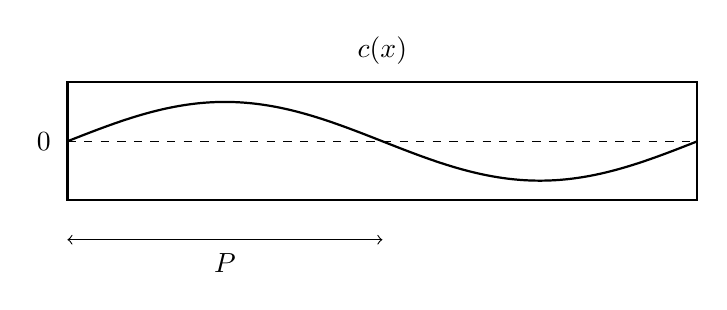
\begin{tikzpicture}[scale=1]
		
		% Rectangle (domaine périodique)
		\draw[thick] (0,0) rectangle (8,1.5);
		
		% Axe x implicite
		\draw[dashed] (0,0.75) -- (8,0.75);
		
		% Courbe périodique c(x)
		\draw[thick,domain=0:8,samples=200]
		plot (\x,{0.75 + 0.5*sin(180*\x/4)});
		
		% Indication de la période P
		\draw[<->] (0,-0.5) -- (4,-0.5);
		\node at (2,-0.8) {$P$};
		
		% Labels
		\node at (4,1.9) {$c(x)$};
		\node at (-0.3,0.75) {$0$};
		
	\end{tikzpicture}
	
	On note $\mathcal{T}\mathcal{}$ l'opérateur de translation de $p$ défini par, pour toute fonction $V$ : $\left(\mathcal{T} v\right)(x) = v(x + P)$ ($v$ est suffisamment régulier).
	
	$\longrightarrow$ \textbf{Nous allons montrer que} $\mathcal{L}_\omega$ et $\mathcal T$ \textbf{commutent}, c'est-à-dire : $\left[\mathcal L_\omega, \mathcal T\right] := \mathcal L_\omega \mathcal T - \mathcal T \mathcal L_\omega = 0$.
	
	C'est à dire pour toute fonction $v$, \fbox{$\mathcal L_\omega\left(\mathcal T v\right) = \mathcal T \left(\mathcal L_\omega v\right)$}.
	
	\begin{enumerate}
		\item[$(1)$] $\begin{aligned}[t]
						\mathcal L_\omega(\mathcal T v)(\lambda)
						&= \mathcal L_\omega(v(\cdot + P))(\lambda) \\
						&= \frac{d}{dx}(c(x)^2 v'(x+P)) + \omega^2 v(x+P) \\
						&= 2c(x)c'(x)v'(x+P) + c(x)^2 v''(x+P) + \omega^2 v(x+P).
					\end{aligned}$
					
					\vspace{.2cm}
					
		\item[$(2)$]  $\begin{aligned}[t]
						\mathcal T \left(\mathcal L_\omega v\right)(x) 
						&= \left(\mathcal L_\omega v\right)(x+P)\\
						&= \frac{d}{dy}\left(c(y)^2v'(y)\right) + \omega^2v(y)\\
						&= 2c'(y)c(y)v'(y) + c(y)^2v''(y) + \omega^2v(y) \\
						&= (2)
					\end{aligned}$
					, où $y = x + p$.
	\end{enumerate} 
	
	Les deux expressions (1) et (2) sont identiques.
	
	\subsection{Invariance translationnelle et ondes de Bloch}
	
	Puisque $\mathcal L_\omega$ et $\mathcal T$ commutent, ils partagent une base de fonctions propres. (cf. théorème spectral pour les opérateurs commutants). Considérons l'espace des solutions $\ker\left(\mathcal L_\omega\right) = \left\{u, \mathcal L_\omega v = 0\right\}$. Il est invariant par $\mathcal T$ et par commutation on peut diagonaliser simultanément :\\
	Il existe des solutions qui sont à la fois dans $\text{Ker}(\mathcal L_\omega)$, et qui sont fonctions propres de $\mathcal T$.\\
	
	\textit{\underline{Remarque :}} Fonction propre de $\mathcal T v = \lambda v, \lambda \in \mathbb{R}$\\
	
	\begin{minipage}{8cm}
	Cela se traduit par : \fbox{$u(x+P) = \lambda u(x)$}.
	\end{minipage}
	\begin{minipage}{8cm}
		\textit{Cette forme correspond à des ondes de Bloch (ondes planes modulées dans le milieu périodique).}
	\end{minipage}
	
	Les solutions sont propagatives si $|\lambda| = 1$ et évanescentes si $|\lambda| \not =  1$.
	
	\subsection{Généralisation aux opérateurs différentiels en dimension N}
	On considère l'opérateur de $\mathbb{R}$ sur $\mathbb{C}^N$ :
	\[
	\mathcal L v = \sum_{k = 0}^n [A]_k(x) \frac{d^k v}{dx^k}, \quad 
	\text{où } 
	\begin{cases}
		\forall x, & [A]_k(x+P) = [A]_k(x),\\
		& [A]_k \text{ : matrice } \mathbb{C}^{N\times N}.
	\end{cases}
	\]

	
	L'opérateur de translation est $\left(\mathcal T v\right)(x) = v(x+P)$. De nouveau, si$\mathcal L et \mathcal T$ commutent , alors ils admettent des fonctions propres (communes) et les solutions $u$ de $\mathcal L v = 0$ peuvent être choisi tels que : $\mathcal T v = \lambda v$ $\implies$ $c(x+P) = \lambda v(x)$ où $\lambda \in \mathbb{C}$ est une valeur propre scalaire de $\mathcal T$.
	\begin{enumerate}
		\item[$(i)$] $\begin{aligned}[t]
						\mathcal L\left(\mathcal T v\right)(x) 
						&= \sum_{k=0}^n [A]_k(x) \frac{d^k}{dx^k}\left(\mathcal T v\right)(x)\\
						&= \sum_{k=0}^n [A]_k(x) \, v^{(k)}(x+P)
					\end{aligned}$\\
		
		\item[$(ii)$] $\begin{aligned}[t]
							\mathcal T\left(\mathcal L v\right)(x) 
							&= \left(\mathcal L v\right)(x+P)\\
							&= \displaystyle\sum_{k=0}^n [A]_k(x+P)v^{(k)}(x+P)\\
							&= (i)
						\end{aligned}$
	\end{enumerate}
	
	Donc $\left[\mathcal L, \mathcal T\right] = 0$.\\
	Les deux précédents opérateurs sont des EDP et concernent des systèmes périodiques continus. Nous allons considérer dans la suite des systèmes discrets.
	
	\subsection{Opérateurs périodiques continus vs. opérateur discrétisés}
	
	Pour simplifier, considérons le système d'ordre $n = 2$.
	\[
	A_2(x)u^{(2)}(x) + A_1(x)u^{(1)} + A_0(x)u(x) = 0
	\]
	
	\vspace{-.5cm}
	
	où les $A_i$ sont des matrices $N\times N$.\\
	On discrétise $x$ sur la grille \[\begin{cases}
		u_n = u(x_n)\\
		x_n = nh
	\end{cases}\] 
	On approxime $u^{(i)}$ par différences finies.
	\[
	u_n^{(1)} = \frac{u_{n+1} - u_{n-1}}{2h} \text { et } u_n^{(2)} = \frac{u_{n+1}-2u_n+u_{n-1}}{h^2}
	\]
	L'opérateur discrétisé devient :
	\[
	A_2(x_n)\left(\frac{u_{n+1}-2u_n+u_{n-1}}{h^2}\right) + A_1(x_n)\left(\frac{u_{n+1}-u_{n-1}}{2h}\right) + A_0(x_n)u_n = 0
	\]
	
	On multiplie par $h^2$ et on regroupe les $u_{n+1}, u_n, u_{n-1}$ et on note $A_1(n) := A(x_n)$.
	
	\[
	\left[A_2(n) + \frac{h}{2} A_1(n)\right]u_{n+1} + \left[h^2A_0(n) - 2A_2(n)\right] u_n + \left[A_2(n) - \frac{h}{2} A_1(n)\right]u_{n-1} = 0
	\]
	
	On note : $B_1(n) = A_2(n) + \frac{h}{2} A_1(n)$, $B_0(n) = h^2A_0(n) - 2A_2(n)$ et $B_{-1}(n) = A_2(n) - \frac{h}{2} A_1(n)$.\\
	
	Puisque $A_k(x+P)  =A_k(x)$, nous avons $A_k(n+M) = A_k(n)$ et donc $B_k(n+M) = B_k(n)$ est $m$-périodique.\\
	
	$\longrightarrow$ \textit{\textbf{On supposera}} que $B_1$ est inversible pour que la récurence soit explicite.\\\\
	Notons $\mathcal T$ l'opérateur de translation discret : $\left(\mathcal T u\right) = u(n-M) := u_{n+1}.$\\
	
	\vspace{-.5cm}
		
	\underline{\textbf{Démontrons que} $\left[\mathcal L, \mathcal T\right] = 0$ :} $\left(\mathcal L v\right)(n) = B_1(n)u_{n+1} = B_0(n)u_n + B_{-1}(n)u_{n-1}$\\
	
	Calculons : $\begin{aligned}[t]
		\mathcal T\left(\mathcal L v\right)(n) 
		&= \left(\mathcal L u\right)(n+M)\\
		&= B_1(n+M)u_{n+M+1} + B_0(n+M)u_{n+M} + B_{-1}(n+M)u_{n+M-1}\\
		\text{\scalebox{0.7}{\textit{où $B$ est périodique  }}} &= B_1(n)u_{n+m-1} + B_0(n)u_{n+M} + B_{-1}(n)u_{n+M-1}\\
		&= \mathcal L\left(\mathcal T v\right)(x) 
	\end{aligned}$
	
	\fbox{
	\begin{minipage}{15cm}
		Les solutions sont donc des ondes de Bloch discrète, c'est-à-dire de la forme :
		
		$u_n = e^{\mu n}\phi(n)$, où :
		\[
		\begin{cases}
			\phi \text{ est } M\text{-périodique }(\text{i.e. } \phi(n+M) = \phi(n))\\
			\mu \in \mathbb{C} \text{ est l\'exposant de Floquet}
		\end{cases}
		\]
	\end{minipage}
	}
	
	Cela implique $\begin{aligned}[t]
		\left(\mathcal T u\right)(n) 
		&:= u_{n+M} \\
		&= e^{\mu(n+M)}\\
		&=  e^{\mu n}e^{\mu M}\phi(n)\\
		&= e^{\mu M}u_n
	\end{aligned}$
	\hspace{1cm} On note \underline{$\lambda = e^{\mu M}$}.
	 
	\hspace{-1cm}\begin{minipage}[t]{20cm}
		Ainsi $\left(\mathcal T u\right)(x) = \lambda u_n$ ce qui revient à dire que c'est un vecteur propre de $\mathcal T$ et $\lambda$ est valeur propre, est dit "Multiplicateur de Floquet".
	\end{minipage}
	
	\subsection{Interprétation des constantes de propagation}
	
	Notation pour le milieu périodique :
	\[
	\begin{cases}
		P = M a\\
		x_n = na
	\end{cases}; u(x_n+P) = u(na+Ma) := u_{n+M}
	\]
	
	\begin{prop}$ $\\
		
		\begin{minipage}{20cm}
		\fbox{
	\begin{minipage}{14.5cm}
		\begin{tabular}{l|l}
			\begin{minipage}{7cm}
				\underline{En 'continue' :}\\
				$u(x+P) = \lambda u(x)$ avec $\lambda = e^{ikP}$\\
				$\iff$\\
				$u(x) = e ^{ikx}\phi(x)$, avec $\phi(x+P) = \phi(x)$\\
				
				où $k\in \left[\frac{-\pi}{P},\frac{\pi}{P}\right] \left(\frac{2\pi}{P}\right)$ "Nombre d'onde"
			\end{minipage}
			& 
			\begin{minipage}{7cm}
				\underline{En 'discret' :}\\
				$u_{n+1} = \lambda u_n$ avec $\lambda = e^{ikMa}$\\
				$\iff$\\
				$u_n = e^{ikna}\phi(n)$, avec $\phi(n+M) = \phi(n)$\\
				
				où $k\in \left[\frac{-\pi}{Ma},\frac{\pi}{Ma}\right] \left(\frac{2\pi}{Ma}\right)$
			\end{minipage}
		\end{tabular}
	\end{minipage}
	} \begin{minipage}{2cm}
	\textcolor{blue}{\textit{Forme des solutions}}
	\end{minipage}
	\end{minipage}
	\end{prop}
	
	\begin{dem}
		\underline{En 'continue' :}\\
		\begin{minipage}[t]{10cm}
			Montrons que (1) $\implies$ (2).\\
		$\begin{aligned}
			u(x) = e^{-ikP}u(x+P) 
			&= e^{ikx} \underbrace{e^{ik(x+P)}u(x+P)}_{\phi(x+P)}\\
			&=e^{ikx} \underbrace{e^{-ikx}\phi(x)}_{\phi(x)}
		\end{aligned}$
		\end{minipage}\begin{minipage}[t]{12.5cm}
			Montrons que $(2) \implies (1)$.\\
		$\begin{aligned}
			u(x+P) 
			&= e^{ik(x+P)}\phi(x+P)\\
			&= e^{ikP}e^{ikx}\phi(x) \text{ , car } \phi \text{ est périodique}\\
			&= \fbox{$e^{ikP}u(x)$}
		\end{aligned}
		$
		\end{minipage}
		
		\vspace{.5cm}
		
		Le cas 'discret' se fait de la même manière.
	\end{dem}
	
	Ces formes de solutions caractérisent la propriété d'une onde se propageant dans un milieu périodique, continu ou discret.
	
	\textbf{\textit{Nous supposerons}} l'existence de cette forme de solution en invoquant le Principe de Floquet-Bloch.
	
	\subsection{Nombre d'onde et constante de propagation}
	
	\begin{enumerate}
		\item[$\cdot$] Si $|\lambda| = 1$ les ondes sont propagatives 
		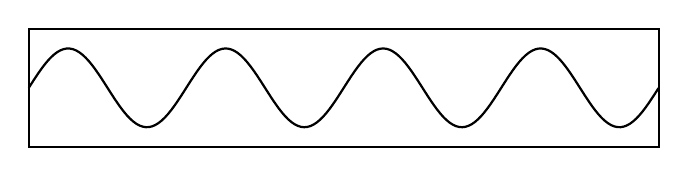
\begin{tikzpicture}[scale=1]
			
			% Rectangle (domaine périodique)
			\draw[thick] (0,0) rectangle (8,1.5);
			
			% Courbe périodique c(x)
			\draw[thick,domain=0:8,samples=200]
			plot (\x,{0.75 + 0.5*sin(180*\x)});
						
		\end{tikzpicture}
		
		\item[$\cdot$] Si $|\lambda| < 1$ les ondes sont évanescentes progressives
		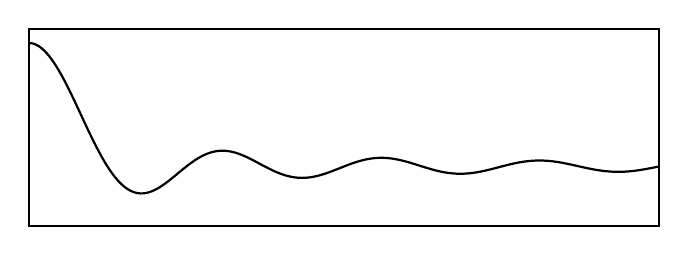
\begin{tikzpicture}[scale=1]
			
			% Rectangle (domaine périodique)
			\draw[thick] (0,0) rectangle (8,2.5);
			
			% Courbe périodique c(x)
			\draw[thick,domain=0.01:8,samples=200]
			plot (\x,{0.75 + 0.5*sin(180*\x)/\x});
			
		\end{tikzpicture}
		
		\item[$\cdot$] Si $|\lambda| > 1$ les ondes sont évanescentes régressive
		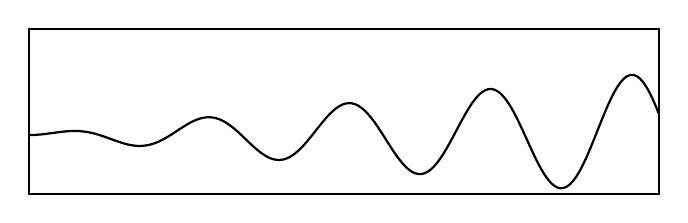
\begin{tikzpicture}[scale=1]
			
			% Rectangle (domaine périodique)
			\draw[thick] (0,0) rectangle (8,2.1);
			
			% Courbe périodique c(x)
			\draw[thick,domain=0.01:8,samples=200]
			plot (\x,{0.75 + 0.1*\x*sin(200*\x)});
			
		\end{tikzpicture}
	\end{enumerate}
	
	\[
	\begin{aligned}
		\text{Comme } u(x + nP) 
		&= \lambda^nu(x) = e^{iknP}u(x) &\text{, or } k = \operatorname{Re}(k) + i\operatorname{Im}(k)\\
		&= e^{-\operatorname{Im}(k)nP}e^{i\operatorname{Re}(k)nP}u(x)
	\end{aligned}
	\]
	
	
	
	\[
	\underbrace{U(x+nP)}_{\textcolor{red}{\text{Translation spatial}}} =\quad
	\underbrace{e^{-\operatorname{Im}(k)nP}}_{\textcolor{red}{\text{Décroissance spatiale}}}\cdot
	\underbrace{e^{i\re(k)nP}}_{\textcolor{red}{\text{Changement de phase}}}\cdot \quad u(x)
	\]
	
	On utilisera les valeurs de $k \in \mathbb{C}$ pour classifier, tracer et interpréter les ondes.
	
	En rappelant que $U(x,t) = \operatorname{Re}\left(u(x,t)e^{-i\omega t}\right)$, on peut donner la forme des solutions dans un milieu $P$-périodique infini comme :\\
	$U(x,t) = U_n(x,t) = \operatorname{Re}\left(u_0(\omega)e^{-i\omega t}\right)$ qui s'écrit d'après le principe de Floquet-Bloch :
	
	\vspace{-.1cm}
	
	\begin{minipage}{6cm}
		\begin{tcolorbox}[colback=white, colframe=red, arc=1mm, boxrule=1pt]
			$U_n(t) = \operatorname{Re}\left(u_0(\omega)e^{i(nkp-\omega t)}\right)$
		\end{tcolorbox}
	\end{minipage} , où $u_0(\omega)$ est l'amplitude de l'onde.\\
	
	\textbf{$\longrightarrow$ Dans la suite}, nous chercherons à trouver les valeurs de $k$ (\textbf{relation de dispersion}) pour différents systèmes périodique (discrets ou continu/discrétisés par éléments finis)
	
	\section{Modélisation dynamique des systèmes périodique discrets}
	
	\subsection{Chaîne monoatomique}
	
	COnsidérons un système infini constitué d'atomes de masse $m$, espacés d'une distance $a$ et reliés par des raideurs linéaires (ressort, quoi) de constante $\beta$.\\
	
	
\includegraphics[scale=.5]{photo1.png}
	
	Ecrivons l'équation d'équilibre d'u atome au point $x_n$ (en l'indice $n$)
	\[
	m\dfrac{d^2U_n}{dt^2} = \displaystyle\sum F_{\text{ext}} = -\beta(U_n-U_{n+1}) - \beta(U_n-U_{n-1}) = \beta(U_{n+1}-2U_n+U_{n-1})
	\]
	
	\textbf{En régime stationnaire} $U_n(t) = u_n(\omega)e^{i\omega t}$.\\
	Principe de Floquet-Bloch : $U_n(t) = u_0(\omega)e^{i(\omega t - kna)}$\\
	
	
	L'équation d'équilibre devient : 
	
	\[
	\begin{aligned}
		m\omega^2 \cancel{U_0e^{i(\omega t - kna)}} 
		&= \beta \left(e^{ika}-2 + e^{-ika}\right)\cancel{U_0e^{i(\omega t - kna)}}\\
		m\omega^2 
		&= \beta \left(e^{ika}-2 + e^{-ika}\right) = 2\beta\left(\frac{e^{ika}+e^ {-ika}}{2}-1\right) = 2\beta\left(\cos(ka)-1\right)\\
		&= - 4\beta \sin^2\left(\frac{ka}{2}\right)
	\end{aligned}
	\]
	
	Donc$\omega^2 = \frac{4\beta}{m}\sin^2\left(\frac{ka}{2}\right)$, en notant $\omega_0 = 2 \sqrt{\frac{\beta}{m}}$, on obtient : \fbox{$\omega = \omega_0\left|\sin\left(\frac{ka}{2}\right)\right|$},\\
	qui est la relation de dispersion, sous la forme $\omega(k)$.\\
	
	\fbox{
	\begin{minipage}[t]{18.5cm}
		\textbf{\underline{Représentation de la solution:}}\\
	
	\begin{minipage}{10cm}
		
\includegraphics[scale=.3]{photo2.png}
	\end{minipage}\begin{minipage}[t]{8cm}
	Comme $k$ est $\frac{2\pi}{a}$-périodique, on ne représente les solution que dans l'intervalle $\left[\frac{-\pi}{a},\frac{\pi}{a}\right]$.
	\end{minipage}
	
	Connaissant le nombre d'onde $k$, on détermine $\begin{cases}
		\text{la vitesse de phase } C_p = \frac{\omega}{k}\\
		\text{la vitesse de groupe } c_z = \frac{\partial \omega}{\partial k}
	\end{cases}$
	
	
\includegraphics[scale=.5]{photo3.png}
	
	$\longrightarrow$ Paquet d'ondes : superposition d'ondes progressives dans un intervalle $k$.
		\end{minipage}}
	
	\vspace{.5cm}
	
	\par \textbf{Cherchons} les solutions complexes $k(\omega)$.
		
	Reprenons : $-\omega^2m = \beta\left(e^{ika}+e^{-ika}-2\right) = 2\beta \left(\frac{e^{-ika}+e^{ika}}{2} - 1 \right)$
	
	$-2\omega^2 = \underbrace{\frac{4\beta}{m}}_{\omega_0^2}\left(\frac{e^{ika}+e^{ika}}{2} - 1\right)$, on introduit : $\begin{cases}
		\lambda = e^{ika}\\
		\lambda^{-1} = e^{-ika}
	\end{cases}$ 
	
	$\dfrac{\lambda+\lambda^{-1}}{2} - 1 + 2 \dfrac{\omega^2}{\omega_0^2} = 0 \implies \fbox{$\lambda^2 + \left(4\dfrac{\omega^2}{\omega_0^2}-2\right)\lambda + 1 = 0$}$
	
	$\Delta = \left(4\dfrac{\omega^2}{\omega_0^2}-2\right)^2-4 = 16\dfrac{\omega^4}{\omega_0^4} - 16 \dfrac{\omega^4}{\omega_0^2} = 16\dfrac{\omega^2}{\omega_0^2}\left[\dfrac{\omega^2}{\omega_0^2} - 1\right]$\\
	
	\begin{minipage}[t]{8cm}
		On reconnais le cas où $\omega \leq \omega_0$ ($\Delta < 0$) :
		
		\[
		\fbox{$
		\lambda = 1 - 2 \dfrac{\omega^2}{\omega_0^2} \pm 2i \dfrac{\omega}{\omega_0}\sqrt{1-\dfrac{\omega^2}{\omega_0^2}}
		$}	
		\]
	\end{minipage}\hspace{1cm}\begin{minipage}[t]{5cm}
	\fbox{\rouge{!}} Si $\lambda_1$ est solution alors $\lambda_2 = \frac{1}{\lambda_1}$ l'est aussi
	\end{minipage}
	
	
	On a 3 cas celons les valeur de $\omega$ et $\omega_0$.
	\begin{enumerate}
		\item Lorsque $\omega > \omega_0$, il n'y a pas de solution propagative, les ondes sont évanescentes :
	\[
	\fbox{
	$
	\lambda = 1 - 2 \dfrac{\omega^2}{\omega_0^2} \pm 2 \dfrac{\omega}{\omega_0} \sqrt{\dfrac{\omega^2}{\omega_0^2}-1}
	$
	}
	\]
	
	Pour retrouver les solutions explicites $k(\omega)$ on peut utiliser : 
	\[
	\begin{aligned}
		\lambda 
		&= e^{ika} = e^{i\left(\re(k)+i\im(k)\right)a} = e^{i\re(k)a}e^{-\im(k)a}\\
		&= e^{-k_I a }\cos(k_R a) + i e^{-ik_I a}\sin(k_R a)
	\end{aligned}
	\]
	
	\item Lorsque $\omega \leq \omega_0$, $\cos(k_Ra) = 1-2\frac{\omega^2}{\omega_0^2}$ et $\sin^2(\frac{k_R a}{2}) = \frac{\omega^2}{\omega_0^2}$.
	
	\item Lorsque $\omega > \omega_0$, on a $\lambda \in \R$, donc $k_R = \pm \frac{\pi}{a} \left[2\pi\right]$.
	\end{enumerate}
	
	\vspace{.5cm}
	
	\par Donc $\lambda = \pm e^{-k_I a} = \pm \left[1-2\frac{\omega^2}{\omega_0^2} \pm2\frac{\omega^2}{\omega_0^2}\sqrt{\frac{\omega^2}{\omega_0^2}-1}\right]$
	
	Donc $k_I = \frac{1}{a}\log\left(-1+2\frac{\omega^2}{\omega_0^2} \pm \frac{2\omega}{\omega_0}\sqrt{\frac{\omega^2}{\omega_0^2}-1}\right)$\\
	
	\textbf{Calcul de :} $\begin{aligned}[t]
		\left(\Omega+\sqrt{\Omega^2-1}\right)
		&= \Omega^2 + 2\Omega\sqrt{\Omega^2 -1} + \Omega^2-1\\
		&=-1 + 2\omega^2+2\Omega\sqrt{\Omega^2-1}
	\end{aligned}$\\
	
	\textbf{Calcul de :} $\begin{aligned}[t]
		\left(\Omega-\sqrt{\Omega^2-1}\right)
		&= \Omega^2 - 2\Omega\sqrt{\Omega^2 -1} + \Omega^2-1\\
		&=-1 + 2\omega^2-2\Omega\sqrt{\Omega^2-1}
	\end{aligned}$
	
	\vspace{.2cm}
	
	\hrule
	
	\vspace{.5cm}
	
	$k_I = \frac{1}{a}\log\left[-1 + 2\frac{\omega^2}{\omega_0^2} - 2\frac{\omega}{\omega_0^2}\sqrt{\frac{\omega^2}{\omega_0^2}-1}\right]$
	
	
\includegraphics[scale=.6]{photo4.png}
	
	\textbf{\underline{Conclusions :}}
	\begin{enumerate}
		\item[$\cdot$] $\omega(k)$ est plus facile à détermier, mais ne donne pas les solutions évanescentes (c'est-à-dire $\im(k)$).
		\item[$\cdot$] $k(\omega)$est plus difficile à calculer mais donne la signification physque de l'évanescence à l'intérieur de la bande interdite.
	\end{enumerate}
	
	\newpage
	
	\subsection{Chaîne di-atomique}
	
		Considérons le système discret périodique à deux atomes :
		
		
\includegraphics[scale=.5]{photo5.png}
		
		Ecrivons l'équation d'équilibre de la cellule unitaire (i.e. l'élément qui, répété, permet de reconstituer toute la chaîne).
		 
		\[
		\begin{aligned}
			m_1\dfrac{d^2U_n}{dt^2} = -\beta\left(U_n-V_n\right) - \beta\left(U_n-V_{n-1}\right)\\
			m_2\dfrac{d^2V_n}{dt^2} = -\beta\left(V_n-U_{n-1}\right) - \beta\left(V_n-U_n\right)
		\end{aligned}
		\]
		
		On considère le régime stationnaire et on applique le principe de Floquet-Bloch : 
		\[
		\begin{aligned}
			u_n = u_0e^{i(\omega t - kna)} = u_0\lambda^n e^{i\omega t}\\
			v_n = v_0 e^{i(\omega t-kna)} = v_0\lambda^ne^{i\omega t}
		\end{aligned}
		\]
		En injectant dans les équations d'équilibre on obtient :
		\[
		\begin{aligned}
			\text{(1) }\omega^2 m_1  U_0 
			&= 2\beta\left(U_0-\frac{V_0}{2}-\frac{1}{\lambda}\frac{V_0}{2}\right)
			\begin{cases}
				u_{n+1} = \lambda u_n\\
				u_{n-1} = \frac{1}{\lambda} u_n
			\end{cases}
			\text{ et }
			\begin{cases}
				v_{n+1} = \lambda v_n\\
				v_{n-1} = \frac{1}{\lambda} v_n
			\end{cases}\\
			\text{(2) }\omega^2 m_2V_0 
			&= 2\beta\left(V_0-U_0-\lambda \frac{U_0}{2}\right)
		\end{aligned}
		\]
		
		$(1)/m_1$ avec $\omega_1 = \sqrt{\frac{2\beta}{m_1}}$ et $(2)/m_2$ avec $\omega_2 = \sqrt{\frac{2\beta}{m_2}}$ :
		$\begin{cases}
			\omega^2U_0-\omega_1^2\left(U_0-\frac{V_2}{2}-\frac{1}{\lambda}\frac{V_0}{2}\right) = 0\\
			\omega^2V_0-\omega_2^2(V_0-\frac{U_0}{2}-\frac{\lambda}{2}U_0) = 0
		\end{cases}$
		
		Ce système  s'écrit sous forme matricielle :
		\[
		\left[\begin{matrix}
			\omega^2 - \omega_1^2 & \frac{\omega_1^2}{2}(1+\frac{1}{\lambda}) \\
			\frac{\omega_2^2}{2}(1+\lambda) & \omega^2-\omega_2^2
		\end{matrix}\right]\left[\begin{matrix}
		U_0\\
		V_0
		\end{matrix}\right] = \left[\begin{matrix}
		0\\
		0
		\end{matrix}\right]
		\]
		
		Les solutions sont non-triviales pour Det = 0 c'est-à-dire :
		\[
		\begin{aligned}
			(\omega^2-\omega_1^2)(\omega^2-\omega_2^2) - \frac{\omega_1\omega_2}{4}(1+\frac{1}{\lambda})(1+\lambda) = 0\\
			\omega^4 - \omega^2(\omega_1^2+\omega_2^2)-\frac{\omega_1^2\omega_2^2}{4}(2+\lambda+\frac{1}{\lambda}) + \omega_1^2\omega_2^2
		\end{aligned}\]
		
		On remarque que $\lambda + \frac{1}{\lambda} = e^{-ika}+e^{ika} = 2 \cos(ka)$\\
		$\omega^4-\omega^2(\omega_1^2+\omega_2^2) - \frac{\omega_1^2\omega_2^2}{4}(\lambda+\frac{1}{\lambda}-2) = 0$.\\
		Donc $\lambda+\frac{1}{\lambda} = 2\cos(ka) - 2 = -4\sin^2(\frac{ka}{2})$.\\
		Ainsi on peut écrire :
		\[
		\omega^4-\omega^2(\omega_1^2+\omega_2^2) - \omega_1^2\omega_2^2\sin^2(\frac{ka}{2}) = 0
		\]
		
		Et $\Delta = (\omega_1^2+\omega_2^2)^2 - \omega_1^2\omega_2^2\sin^2(\frac{ka}{2})$ positif car $\sin ^2 \leq 1$ et $(\omega_1^2-\omega_2^2)^2 \geq 0$.\\
		Les deux solutions s'écrivent :
		\[
		\omega^2(k) = \beta \left(\frac{1}{m_1}+\frac{1}{m_2}\right) \pm \beta \sqrt{\left(\frac{1}{m_1}+\frac{1}{m_2}\right)^2-\frac{4\sin^2(\frac{ka}{2})}{m_1m_2}}
		\]
		on introduit $\omega_3 = \sqrt{2\beta\left(\frac{1}{m_1}+\frac{1}{m_2}\right)} =: \omega_{max}$.\\
		
		
\includegraphics[scale=.5]{photo6.png}
		
		Si on suppose que $m_1=m_2$, la relation de dispersion devient : $\omega^2(k) = \omega_1^2(1\pm\cos(\frac{ka}{2}))$.\\
		Intéressons-nous désormais aux propriétés de l'ondes à l'intérieur de la bande interdite :\\
		Reprenons la relation de dispersion :
		\[
		\begin{cases}
			\omega^2U_0 = \omega_1^2\left(U_0-\frac{V_2}{2} -\frac{1}{\lambda}\frac{V_0}{2}\right) & /\omega_1 ^2 \text{ et } \Omega_1 ^2 = \frac{\omega^2}{\omega_1^2} \\
			\omega^2V_0 = \omega_2^2(V_0-\frac{U_0}{2} -\frac{\lambda}{2}U_0) & /\omega_2^2 \text{ et } \Omega_2^2 = \frac{\omega^2}{\omega_2^2}
		\end{cases}
		\begin{cases}
			(2\Omega_1^2-2)U_0 + (1+\frac{1}{\lambda})V_0 = 0 \\
			(1+\lambda)U_0+(2\Omega_2^2-2)V_0 = 0
		\end{cases}
		\]
		
		On annuler le déterminant :
		\[
		\begin{aligned}
			(2\Omega_1^2-2)(\Omega_2^2-2) - \underbrace{(1+\frac{1}{\lambda})(1+\lambda)}_{\rouge{4\sin^2(\frac{ka}{2})}} = 0\\
			\lambda - \underbrace{\left[4(\Omega_1^2-1)(\Omega_2^2-1) +2\right]}_{2(1-2(\Omega_1^2-1)(\Omega_2^2-1))} + \frac{1}{\lambda} = 0\\
			\Delta = 16(\Omega_1 ^2-1)(\Omega_2^2-1)\left[\underbrace{(\Omega_1^2-1)(\Omega_2^2-1)}_{\rouge\Gamma}-1\right]
		\end{aligned}
		\]
		
		Les solutions complexes sont alors :
		\[
		\lambda = (2\Gamma-1)\pm2\sqrt{(\Omega_1^2-1)(\Omega_2^2-1)(\Gamma-1)}
		\]
		
		\fbox{
		\begin{minipage}[t]{15cm}
			Ce qui donne la solution $k(\omega)$ explicite :
		\[
		k(\omega) = \frac{i}{a}\log\left[\frac{1}{\omega_1^2\omega_2^2}\left(2\omega^4-2\omega^2\omega_3^2 + \omega_1 ^2\omega_2^2 + 2\omega\sqrt{(\omega^2-\omega_1^2)(\omega^2-\omega_2^2)(\omega^2-\omega_3^2)}\right)\right]
		\]
		\end{minipage}}


		\hspace{-.5cm}
\includegraphics[scale=.4]{photo7.png}
	
	\subsection{Généralisation aux systèmes à plusieurs degrés de liberté (DDL)}
	
	On considère une chaîne masse-ressort :
	
	
\includegraphics[scale=.5]{photo11.png}
	
	L'équation d'équilibre en régime harmonique s'écrit en $U_n$ :
	
	\[m_n\dfrac{d^2U_n}{dt^2} = -\beta_n(U_n-U_{n+1}) - \beta_{n-1}(U_n-U_{n-1})\]
	
	qui s'écrit : $m_n \overset{\textbf{..}}{U}_n - \beta_{n-1}U_{n-1} + (\beta_n+\beta_{n-1})U_n - \beta_nU_{n+1} = 0$.\\
	Le système s'écrit sous forme matricielle :
	\[\left[\begin{matrix}
		\ddots & & & & \\
		& m_{n-1} & & (0) & \\
		& & m_n & & \\
		&(0) & & m_{n+1} & \\
		& & & & \ddots
	\end{matrix}\right]\left[\begin{matrix}
	\vdots\\
	\overset{\textbf{..}}{U}_{n-1}\\
	\overset{\textbf{..}}{U}_{n}\\
	\overset{\textbf{..}}{U}_{n+1}\\
	\vdots
	\end{matrix}\right] + \left[\begin{matrix}
	\ddots & & & & \\
	& \ddots & & & \\
	(0) & - \beta_{n-1} & \beta_{n+1}+\beta_n & -\beta_n & (0)\\
	& & & \ddots & \\
	& & & & \ddots
	\end{matrix}\right]\left[\begin{matrix}
	\vdots\\
	U_{n-1}\\
	U_n\\
	U_{n+1}\\
	\vdots
	\end{matrix}\right] = \left[\begin{matrix}
	0 \\
	\vdots \\
	\vdots \\
	\vdots \\
	0
	\end{matrix}\right]\]
	
	C'est une EDO qui s'écrit : 
	\begin{center}
		\begin{minipage}{4cm}
			\enc{red}{$\mathbb{M}\dfrac{\partial^2 \overset{\rightarrow}{U}}{\partial t^2} + \mathbb{K} \overset{\rightarrow}{U} = \overset{\rightarrow}{0}$}
		\end{minipage}
	\end{center}
	
	On \textbf{nomme} \underline{$\mathbb{M}$ la \textbf{matrice de masse}} et \underline{$\mathbb{K}$ la \textbf{matrice de raideur}}.
	
	\newpage
	
	On peut représenter l'écriture des matrices $\mathbb{K}$ et $\mathbb{M}$ du système comme un "assemblage" d'éléments discrets (raideurs 1D) qui sont des cellules :\\
	\newlength{\x}
	\setlength{\x}{1cm}
	\newlength{\y}
	\setlength{\y}{1.5cm}
	\[\mathbb{K} = \left[\begin{matrix}
		-\beta_{n-1} & \beta_{n-1}+\enc[\x]{red}{$\beta_n$} & \enc[\y]{red}{$-\beta_n$} & 0 &  \\
		0 & \enc[\y]{red}{$-\beta_n$} & \enc[\x]{red}{$\beta_n$} + \enc[\y]{blue}{$\beta_{n+1}$} & \enc[1.8cm]{blue}{$-\beta_{n+1}$} & 0 \\
		& 0 & \enc[\y]{blue}{$\beta_{n+1}$} & \enc[\y]{blue}{$\beta_{n+1}$} + \beta_{n+2} & - \beta_{n+2}
	\end{matrix}\right]\]
	
	Cela permet d'écrire de façon plus rapide les matrices (EDO) d'un système périodique :
	
	\begin{ex}\begin{minipage}{15cm}
			
\includegraphics[scale=.5]{photo12.png}
		\end{minipage}
		
		Écrire le système (EDO) sous la forme $\mathbb{M}\overset{\textbf{..}}{U} + \mathbb{K}U = 0$.
		
		\begin{minipage}[t]{19.5cm}
			\textbf{\underline{Rappel :}} \begin{minipage}{3cm}
				
\includegraphics[scale=.5]{photo13.png}
			\end{minipage} le système est : $\left[\begin{matrix}
			m_1 & 0 \\
			0 & m_2
		\end{matrix}\right] \left[\begin{matrix}
		\overset{\textbf{..}}{U} \\ 
		\overset{\textbf{..}}{V}
		\end{matrix}\right] + \left[\begin{matrix}
		k & -k \\
		-k & k
		\end{matrix}\right]\left[\begin{matrix}
		U \\
		V
		\end{matrix}\right] = \left[\begin{matrix}
		0 \\ 0
		\end{matrix}\right]$.
		\end{minipage}
		
		\vspace{.5cm}
		
		\[
		\left[\begin{matrix}
			\rouge{m_1} & 0 & 0 & 0 \\
			0 & m_2 & 0 & 0 \\
			0 & 0 & m_3 & 0 \\
			0 & 0 & 0 & m_4
		\end{matrix}\right]\left[\begin{matrix}
		\overset{\textbf{..}}{U_1} \\ \overset{\textbf{..}}{U_2} \\ \overset{\textbf{..}}{U_3} \\ \overset{\textbf{..}}{U_4}
		\end{matrix}\right] + \left[\begin{matrix}
		\rouge{k_1} + k_4 & \rouge{-k_1} & 0 & -k_4 \\
		\rouge{-k_1} & \rouge{k_1}+\bleu{k_2} & \bleu{-k_2} & 0 \\
		0 & \bleu{-k_2} & \bleu{k_2} + \vert{k_3} & \vert{-k_3} \\
		-k_4 & 0 & \vert{-k_3} & \vert{k_3} + k_4
		\end{matrix}\right]\left[\begin{matrix}
		U_1 \\ U_2 \\ U_3 \\ U_4
		\end{matrix}\right] = \left[\begin{matrix}
		0 \\ 0 \\ 0 \\ 0
		\end{matrix}\right]
		\]
		
		En régime stationnaire , $\mathbb{M}\overset{\rightarrow}{\overset{\textbf{..}}{U}} + \mathbb{K}\overset{\rightarrow}{U} = \overset{\rightarrow}{0}$ devient : $ \underbrace{\left(\mathbb{K}-\omega^2\mathbb{M}\right)}_{\rouge{\mathbb{D}}}\overset{\textbf{..}}{U} = 0$. Où $\rouge{\mathbb{D}}$ est la raideur dynamique.		
	\end{ex}
	
	
	\begin{ex}\begin{minipage}{18cm}
			
\includegraphics[scale=.5]{photo14.png}
		\end{minipage}
		
		\begin{enumerate}
			\item Écrire les matrices $\mathbb{K}, \mathbf{M}$ d'une cellule périodique "bords libres".
			
			\[
			\underbrace{\left[\begin{matrix}
				\frac{m_1}{2} & 0 & 0 \\
				0 & m_2 & 0 \\
				0 & 0 & \frac{m_1}{2}
			\end{matrix}\right]}_{\mathbb{M}}\left[\begin{matrix}
			\overset{\textbf{..}}U_L \\ \overset{\textbf{..}}U_i \\ \overset{\textbf{..}}U_R 
			\end{matrix}\right] + \underbrace{\left[\begin{matrix}
			\rouge{k_1} & \rouge{-k_1} & 0 \\
			\rouge{-k_1} & \rouge{k_1} + \bleu{k_2} & \bleu{-k_2} \\
			0 & \bleu{-k_2} & \bleu{k_2}
			\end{matrix}\right]}_{\mathbb{K}}\left[\begin{matrix}
			U_L \\ U_i\\ U_R
		\end{matrix}\right] = \left[\begin{matrix}
		0 \\ 0 \\ 0
		\end{matrix}\right]
			\]
			
			qui s'écrit : $\left(\mathbb{K}-\omega^2\mathbb{M}\right)\left[\begin{matrix}
				U_L \\ U_i \\ U_R
			\end{matrix}\right] = \left[\begin{matrix}
				0 \\ 0 \\ 0
			\end{matrix}\right]$.
			
			Utilisons $\mathbb{K}$ et $\mathbb{M}$ pour écrire l'EDO du système "généralisé" : 
			
			\[\left(\left[\begin{matrix}
				\bleu{k_1}+\bleu{k_2} & \bleu{-k_2} & & \\
				\bleu{-k_2} & k_1 + \bleu{k_2} & -k_1 & 0 \\
				& -k_1 & k_1+k_2 & -k_2 \\
				& 0 & -k_2 & k_2+k_1
			\end{matrix}\right] -\omega^2\left[\begin{matrix}
			\bleu{m_2} & & & \\
			& \frac{m_1}{2}+\bleu{\frac{m_1}{2}} & & \\
			& & m_2 & \\
			& & & \frac{m_1}{2}+\frac{m_1}{2}
			\end{matrix}\right]\right)\left[\begin{matrix}
			\vdots\\
			\left[\begin{matrix}
			U_L^{(n)}\\
			U_i^{(n)}
			\end{matrix}\right] \\
			\vdots
			\end{matrix}\right] = \left[\begin{matrix}
			\vdots\\
			\left[\begin{matrix}
				0\\
				0
			\end{matrix}\right] \\
			\vdots
			\end{matrix}\right]\]
			
			
			On obtient :
			
			\[
			\left(\left[\begin{matrix}
				0 & -k_2 & k_1 + k_2 & -k_1 & 0& 0 \\
				0 & 0 & -k_1 & k_1 + k_2 & -k_2 & 0
			\end{matrix}\right]-\omega^2\left[\begin{matrix}
			0 & 0 & m_1 & 0 & 0 & 0 \\
			0 & 0 & 0 & m_2 & 0 & 0
			\end{matrix}\right]\right)\left[\begin{matrix}
			U_L^{(n-1)} \\
			U_i^{(n-1)} \\
			U_L^{(n)} \\
			U_i^{(n)} \\
			U_L^{(n-1)} \\
			U_i^{(n-1)}
			\end{matrix}\right] = \left[\begin{matrix}
			0 \\
			\vdots \\
			0
			\end{matrix}\right]
			\]
		\end{enumerate}
		
		
\includegraphics[scale=.5]{photo15.png}
	\end{ex}
	
	
	\begin{ex}[Poutre d'Euler-Bernoulli] Éléments discrets\\
		\begin{minipage}{7cm}
			
\includegraphics[scale=.5]{photo16.png}\\
			$\rho$ : densité volumique \\
			$A$ : Section \\
			$L$ : longueur \\
			$I$ : Moment de section \\
			$E$ : Module de Young
		\end{minipage} $ \begin{aligned}
		\mathbb{M}_e =& \dfrac{\rho A L}{420}\left[\begin{matrix}
			156 & 22L & 54 & -13L \\
			& 4L^2 & 13L & -3L^2 \\
			& & 156 & -22L \\
			 & & & 4L^2
		\end{matrix}\right] \\
		\mathbb{K}_e =& \dfrac{2EI}{L}\left[\begin{matrix}
			6 & 3L & -6 & 3L \\
			  & 2L^2 & -3L & L^2 \\
			  &     & 6 & -3L \\
			(Sym) &   &   & 2L^2
		\end{matrix}\right]
		\end{aligned} $
		
		On peut décomposer nos matrices élémentaires en deux "domaines" (c'est-à-dire $U_L, U_R$) : $\mathbb{M}_e = \left[\begin{matrix}
			M_L & M_{LR} \\
			M_{RL} & M_R
		\end{matrix}\right]$ et $\mathbb{K}_e = \left[\begin{matrix}
		K_L & K_{LR} \\
		K_{RL} & K_R
		\end{matrix}\right]$.\\
		\begin{minipage}[t]{18cm}
			Où, par symétrie de $\mathbb{M}_e$ et $\mathbb{K}_e$ : $\begin{cases}
			M_L = M_L^T & \text{ (idem pour } M_R, K_L, K_R) \\
			M_{LR} = M_{RL}^T & \text{ (idem pour } K_{LR} = K_{RL}^T)
		\end{cases}$\\
		
		On note alors les raideurs dynamiques : $D_{i,j} = K_{i,j}-\omega^2M_{i,j}$, $i,j \in \{L,R\}$.
		\end{minipage}
		
		\underline{Le système initial :} 
		
		\vspace{.5cm}
		
		\begin{minipage}[t]{18.5cm}
			$\left(\mathbb{K}_e-\omega^2\mathbb{M}_e\right)\overset{\rightarrow}{U} = 0$ alors : $\left[\begin{matrix}
		D_L & D_{LR} \\
		D_{RL} & D_R
		\end{matrix}\right]\left[\begin{matrix}
		\overset{\rightarrow}{U_L} \\ \overset{\rightarrow}{U_R}
		\end{matrix}\right] = \left[\begin{matrix}
		0 \\ 0
		\end{matrix}\right]$, où $\overset{\rightarrow}{U_L} = \left[\begin{matrix}
		V_L \\ \Theta_L
		\end{matrix}\right]	$ et $\overset{\rightarrow}{U_R} = \left[\begin{matrix}
		V_R \\ \Theta_R
		\end{matrix}\right]	$
		\end{minipage}
		
		\begin{minipage}[t]{16cm}
			Écrivons l'assemblage de deux cellules décrites par leur matrice de raideur dynamique : $\mathbb{D} = \left[\begin{matrix}
			D_L & D_{LR} \\
			R_{RL} & D_R
		\end{matrix}\right]$ \begin{minipage}{5cm}
		
\includegraphics[scale=.5]{photo17.png}
		\end{minipage}
		\end{minipage}
		
		\[
		\left[\begin{matrix}
			\rouge{D_L} & \rouge{D_{LR}} & \\
			\rouge{D_{RL}} & \rouge{D_R}+D_L & D_{LR} \\
			& D_{RL} & D_R
		\end{matrix}\right]\left[\begin{matrix}
		U_L^{n-1} \\ U_L^n \\ U_L^{n+1}
		\end{matrix}\right] = \left[\begin{matrix}
		0 \\ 0 \\ 0
		\end{matrix}\right]
		\]
		Pour un assemblage "infini" de cellules :\\
		\begin{minipage}[t]{18.5cm}
			$\left[\begin{matrix}
			\ddots & \ddots & \ddots & & & & \\
			& D_{RL} & D_L+D_R & D_{LR} & & & & \\
			& \ddots & \ddots & \ddots & & & \\
			& & D_{RL} & D_L+D_R & D_{LR} & & \\
			& & & \ddots & \ddots & \ddots & \\
			& & & & D_{RL} & D_L + D_R & D_{LR} \\
			& & & & \ddots & \ddots & \ddots
		\end{matrix}\right]\left[\begin{matrix}
		\vdots \\
		U_{n-1} \\
		U_n\\
		U_{n+1} \\
		\vdots
		\end{matrix}\right] = \left[\begin{matrix}
		\vdots \\ \vdots \\ 0 \\ \vdots \\ \vdots
		\end{matrix}\right]$
		\end{minipage}
	\end{ex}
	
	
	
	
	
	
	
	
	
	
	
	
	
	
	
	
	
	
	
	
	
	
	
	
	
	
	
	
	
	
	
	
	
	
	
	
	
	
	
	
	
	
	
	
	
	
	
	
	
	
	
	
	
	
	
	
	
	
	
	
	
	
	
	
	
	
	
	
	
	
	
	
	
	
	
	
	
	
	
	
	
	
	
	
	
	
	
	
	
	
	
	
	
	
	
	
	
	
	
	
	
	
	
	
	
	
	
	
	\newpage
	
	\section{TD}
	
	\begin{exo}[Système périodique et résonance locale]$ $\\
		\textbf{\underline{Rappel démarche :}}
		
		\vspace{-.5cm}
		
	\begin{minipage}[t]{18.5cm}
	\begin{enumerate}
		\item Identifier la période (cellule périodique minimale du système)
		\item  Écrire les équations d'équilibre (opérateur $\m L U(x,t) = 0$) pour chaque degré de liberté
		\item Invoquer la stationnarité ($U(x,t) \to u(x,\omega)$) puis le principe de Floquet-Bloch :
		\[(u_{n+1},u_{n-1},\ldots, \to \left(\lambda,\frac{1}{\lambda}\right)u_n) \text{ où } u_n(t) = u_0 e^{i(nka-\omega t)}\]
		\item Équation l'équation de dispersion (ou système $\to \det = 0$) liant $\omega$ et $\lambda$.
		\item Résoudre $((i)$ $\omega(k),$ (ii) $k(\omega))$
		\item Interpréter les solutions $\left(\left[\begin{minipage}{2.5cm}
			\text{propagatives}\\\text{évanescentes}
		\end{minipage}\right] et \left[\begin{minipage}{3cm}
			\text{progressive + }$x$\\\text{régressive + }$x$
		\end{minipage}\right]\right)$ et tracer.
	\end{enumerate}
	\end{minipage}
	
	
	
\includegraphics[scale=.5]{photo8.png}
	
	On produit des bandes interdites sous forme "additive".\\
	Si $m_2\to 0$, on doit retrouver la chaîne mono-atomique.
	\end{exo}
	
	\begin{sol}$ $
		
		\vspace{-.5cm}
		
	\begin{enumerate}
		\item On identifie la période : 
\includegraphics[scale=.2]{photo9.png} 
	
		\item On écrit les équations d'équilibre :
		\[\begin{aligned}
			\text{(1) }&m_1\dfrac{d^2 U_n}{dt^2} &=& -\beta_1(U_n-U_{n+1})-\beta_1(U_n-U_{n-1}) - \beta_2(U_n-V_n)\\\\
			\text{(1) }&m_1\dfrac{d^2 U_n}{dt^2} &= &\beta_1(U_{n+1}-2U_n+U_{n-1}) + \beta_2(V_n-U_n)\\\\
			\text{(2) }& m_2\dfrac{d^2 V_n}{dt^2} &= &\beta_2(U_n-V_n)
		\end{aligned}\]
		
		\item On considère le régime stationnaire et le principe de Floquet-Bloch : $U_n = U_0\lambda^n e^{i\omega t}$ et $V_n = V_0 \lambda^n e^{i\omega t}$. Et on réécrit les 2 équations :
		\[\begin{aligned}
			\text{(1) } -m_1\omega^2 U_0 &= \beta_1(\lambda U_0 - 2U_0 + \frac{1}{\lambda}U_0)+\beta_2(V_0-U_0)\\
			\text{(2) } -m_2 \omega^2 V_0 &= \beta_2(U_0-V_0)
		\end{aligned} \]
		
		Puis, on divise $(i)$ par $m_i$ :
		\[\begin{aligned}
			-\omega^2 U_0 &= \frac{\beta_1}{m_1}(\lambda U_0 - 2U_0 + \frac{1}{\lambda}U_0)+\frac{\beta_2}{\beta_1}\frac{\beta_1}{m_1}(V_0-U_0)\\
			-\omega^2 V_0 &= \beta_2/m_2(U_0-V_0)
		\end{aligned} \]
		
		\begin{minipage}[t]{18cm}
			On regroupe selon $U_0$ et $V_0$ et on utilise les notations suivantes : $\omega_1=\sqrt{\frac{\beta_1}{m_1}}$, $\omega_2 = \sqrt{\frac{\beta_2}{\beta_1m_2}}$ et $r = \frac{\beta_2}{\beta_1}$  :
		\end{minipage}
		\[ \begin{aligned}
			(\omega^2 + \omega_1^2(\lambda+\frac{1}{\lambda}-2)-r\omega_1^2)U_0&+&r\omega_1^2 V_0&=0\\
			\omega_2^2 U_0&+&(\omega^2-\omega_2^2)V_0 &=0
		\end{aligned} \]

		
		On pose : $A = \left[\begin{matrix}
			\omega^2 + \omega_1^2(\lambda+\frac{1}{\lambda}-2-r) & r\omega_1^2\\
			\omega_2^2 & \omega^2-\omega_2^2
		\end{matrix}\right]$ et on a ainsi : $AX = 0$ où $X = \left[\begin{matrix}
		U_0\\ V_0
		\end{matrix}\right]$.
		
		Regardons le déterminant pour trouver une condition nécessaire et suffisante pour trouver des solutions non trivial :
		\[\begin{aligned}
			&\det A = 0\\
			\iff&\left[\omega^2 + \omega_1^2(\lambda+\frac{1}{\lambda}-2-r)\right]\times (\omega^2-\omega_2^2) - r\omega_1^2\omega_2^2 =0\\
			\iff & \omega^4 + \omega^2 \left[\omega_1^2(\lambda+\frac{1}{\lambda}-2-r)-\omega_2^2\right]-w_1^2w_2^2\left[r+\lambda+\frac{1}{\lambda}-2-r\right] = 0\\
			\iff&\omega^4 + \omega^2 \left[\omega_1^2(\lambda+\frac{1}{\lambda}-2-r)-\omega_2^2\right]-w_1^2w_2^2\left[\lambda+\frac{1}{\lambda}-2\right] = 0\\
			\iff&\omega^4 + \omega^2 \left[\omega_1^2\left(2\left[cos(ka)-1\right]-r\right)-\omega_2^2\right]-2w_1^2w_2^2\left(\cos(ka)-1\right) = 0
		\end{aligned}\]
		
		Puis on regarde le discriminant :
		\[\begin{aligned}
			\Delta &=\left[\omega_1^2\left(2\left[cos(ka)-1\right]-r\right)-\omega_2^2\right]^2+8w_1^2w_2^2\left(\cos(ka)-1\right)\\
			&=\left[2\omega_1^2\left[cos(ka)-1\right]-\omega_2^2-\omega_1^2 r\right]^2+8w_1^2w_2^2\left(\cos(ka)-1\right)\\
			&=\left[2\omega_1^2\left[cos(ka)-1\right]-\omega_2^2\right]^2+\omega_1^4 r^2+8w_1^2w_2^2\left(\cos(ka)-1\right)\\
			&=\cdots\\
			\Delta&>0
		\end{aligned}\]
	\end{enumerate}
	
	\newpage
	
	\textbf{\underline{Tracé des solutions :}} Il y a 2 cas : $\begin{cases}
		\omega_2 <2\omega_1\\
		\omega_2 = 2 \omega_1\\
		\omega_2 > 2\omega_1
	\end{cases}$ :
	
	
\includegraphics[scale=.5]{photo10.png}
	
	Pour calculer le $k$ complexe dans la bande interdite, on doit résoudre $k(\omega)$. L'équation de dispersion peut se réécrire en notant : $\Omega_1^2 = \frac{\omega^2}{\omega_1^2}$ et $\Omega_2^2 = \frac{\omega^2}{\omega_2^2}$ :
	
	\[\implies  \lambda^2 + \left[\Omega_1^2+r\dfrac{\Omega_2^2}{1-\Omega_2^2}-2\right]+1 = 0\]
	
	\[k(\omega) = \frac{i}{a}\log\left[1-\frac{\Omega_1^2}{2}-\frac{r}{2}\frac{\Omega_2}{1-\Omega_2^2} \pm \sqrt{\left(\Omega_1^2+\frac{r\Omega_2^2}{1-\Omega_2^2}\right)\left(\Omega_1^2+\frac{r\Omega_2^2}{1-\Omega_2^2}-4\right)}\right]\]
	\end{sol}
	
	\begin{exo}[Formulation matricielle]
		\begin{minipage}[t]{15cm}
			Appliquer à la chaîne monoatomique, en considérant la cellule périodique :
		\end{minipage}
		
		
\includegraphics[scale=.5]{photo18.png}.
		
		\begin{enumerate}
			\item Déterminer les matrices de masses et raideurs :
			\[
			\mathbb{K}_e, \mathbb{M}_e \text{ puis } \mathbb{D} = \left[\begin{matrix}
				D_L & D_{RL}\\
				D_{RL} & D_R
			\end{matrix}\right]
			\]
			
			\item Ecrire la matrice globale du système infini.
			
			\item Appliquer le principe de Floquet-Bloch ($U_{n+1}$ et $U_{n-1}$ en fonction de $U_n$ et $\lambda$) et en déduire l'équation de dispersion.
		\end{enumerate}
	\end{exo}
	
	\begin{sol}$ $\\
		\begin{enumerate}
			\item $\mathbb{M}_e = \left[\begin{matrix}
				\frac{m}{2} & 0 \\
				0 & \frac{m}{2}
			\end{matrix}\right]$ et $\mathbb{K}_e=\left[\begin{matrix}
				K & -K \\
				-K & K
			\end{matrix}\right]$\\
			$\mathbb{D} = k_e-\omega^2\mathbb{M}_e = \left[\begin{matrix}
				k-\omega^2\frac{m}{2} & -k \\
				-k & k-\omega^2\frac{m}{2}
			\end{matrix}\right] = \left[\begin{matrix}
				D_L & D_{LR} \\
				D_{RL} & D_R
			\end{matrix}\right]$
			
			\item $\left[\begin{matrix}
				\ddots & \ddots & \ddots \\
				& -K & 2K-\omega^2m & -K \\
				& & \ddots & \ddots & \ddots 
			\end{matrix}\right]\left[\begin{matrix}
				\vdots \\ U_{n-1} \\ U_n \\ U_{n+1} \\ \vdots
			\end{matrix}\right] = \left[\begin{matrix}
				\vdots \\
				0 \\
				\vdots
			\end{matrix}\right]$
			
			\item \begin{minipage}[t]{18.5cm}
				Floquet-Bloch donne $\begin{cases}
				U_{n+1} = \lambda U_n \\
				U_{n-1} = \frac{1}{\lambda} U_n
			\end{cases}$ et $-KU_{n-1} + (2K-\omega^2n)U_n-KU_{n+1} = 0$
			\end{minipage}
			
			On en déduit l'équation de dispersion des ondes : 
			\[
			\left(-K\frac{1}{\lambda} + (2K-\omega^2m)-K\lambda\right)U_n = 0
			\]
			
			\begin{minipage}[t]{15cm}
				$\div(-K) \implies \left(\lambda + \omega^2\frac{m}{K} -2+\frac{1}{\lambda}\right)U_n = 0 \to $ Équation de dispersion
			\end{minipage}
			
			\begin{minipage}[t]{15cm}
				La forme $D_{RL}U_{n-1}+(D_L+D_R)U_n+D_{LR}U_{n+1} = 0$ est générale (elle s'applique à toute cellule périodique décrite par une raideur dynamique $\mathbb{D} = \left[\begin{matrix}
				D_L & D_{LR} \\
				D_{RL} & D_R
			\end{matrix}\right]$)
			\end{minipage}
			
			\enc{red}{La relation de dispersion est alors :
			
			\[
			\left(\frac{1}{\lambda} D_{RL} + (D_L+D_R)+D_{LR}\lambda\right)\overset{\textbf{..}}{U_n} = 0_{p,1} \text{ (1)}
			\]
			}
			
			\textbf{Note :} \begin{minipage}[t]{15cm}
				C'est un problème aux valeurs propres de dimension notée $p$, polynomiak, d'ordre 2. Il admet donc (en général) $2p$ solutions :
				\begin{enumerate}
					\item[$p$] solutions où $\abs{\lambda} < 1$ (progressives)
					\item[$p$] soltuions où $\abs{\lambda} > 1$ (régressives)
				\end{enumerate}
			\end{minipage}
		\end{enumerate}
	\end{sol}
	
	\newpage
	
	\begin{ex}[Suite de l'exercice précédent] $ $\\
		Écrire (1) sous la forme $\omega(k)$ c'est-à-dire : $(A-\omega^2B)\emptyset = 0$.
	\end{ex}
	\begin{sol}
		\[\begin{aligned}
			\left(\frac{1}{\lambda}D_{RL}+(D_L+D_R)+\lambda D_{LR}\right)U_n = 0 \\
			\left[\frac{1}{\lambda}(K_{RL}-\omega^2M_{RL})+(K_L-\omega^2M_L)+(K_L-\omega^2M_L+K_R-\omega^2M_R)+\lambda(K_{LR}-\omega^2M_{LR})\right]U_n = 0\\
			\left(\underbrace{\left[\frac{1}{\lambda}K_{RL}+K_L+K_R+\lambda K_{LR}\right]}_{\overset{\sim}{K}(\lambda)}-\omega^2\underbrace{\left[\frac{1}{\lambda}M_{RL}+M_L+M_R+\lambda M_{LR}\right]}_{\overset{\sim}{M}(\lambda)}\right)U_n = 0
		\end{aligned}\]
		
		\begin{minipage}[t]{18cm}
			Le problème aux VP devient : \enc[5.5cm]{red}{$\left[\overset{\sim}{K}(\lambda) - \omega^2\overset{\sim}{M}(\lambda)\right]U_n = 0$} (2) forme $\omega(\lambda)$
		\end{minipage}
		
		En pratique : \begin{minipage}[t]{15cm}
			
			\vspace{-.3cm}
			
			\begin{enumerate}
				\item donne des solutions complexes ($\lambda \in \C$) pour $\omega$ réel donné.
				\item donner des solutions réelles ($\omega \in \R^*$) pour $k$ réel donné ($k \to \lambda = e^{iak}$).
			\end{enumerate}
			Sa résolution s'apparente au calcul de modes propres/fréquences propres.
		\end{minipage}
	\end{sol}
	
	\begin{exo}[Exo type d'examen] $ $\\
		On considère la cellule périodique suivante :\\
		
		\begin{minipage}{6cm}
			
\includegraphics[scale=.5]{photo19.png}
		\end{minipage}\begin{minipage}{15cm}
		\begin{enumerate}
			\item Ecrire le système d'EDP en $U_n$ et $V_n$.
			\item En déduire l'équation de dispersion.
			\item Choisir une cellule périodique et écrire $\mathbb{K}_e$, $\mathbb{M}_e$ pour $\mathbb{D}$.
			\item Retrouver directement d'équation de dispersion (matricielle).
		\end{enumerate}
		\end{minipage}
	\end{exo}
	
\end{document}